\documentclass[letterpaper, 12pt]{article}

\usepackage{geometry}
 \geometry{
 letterpaper,
 total={170mm,257mm},
 left=20mm,
 top=20mm,
 bottom=20mm
 }
\usepackage{graphicx} % Required for inserting images
\usepackage{authblk}
\usepackage{amssymb}
\usepackage{lipsum}
\usepackage{float}
\usepackage{times}
\usepackage{amsmath}
\usepackage[format=plain,
            labelfont={bf,it},
            textfont=it]{caption}
\captionsetup{justification=raggedright,singlelinecheck=false}
\usepackage{ragged2e}
\usepackage{longtable}
\usepackage{comment}
\usepackage{setspace}
\usepackage{fancyhdr}
\usepackage{titlesec}
\usepackage[hyperindex,breaklinks]{hyperref}
\hypersetup{
    colorlinks=true,
    linkcolor=blue,
    filecolor=magenta,      
    urlcolor=blue,
    pdftitle={Overleaf Example},
    pdfpagemode=FullScreen,
    }
% \usepackage{background} % add COSIG logo to page
\usepackage[T1]{fontenc}
\usepackage{helvet}
\renewcommand{\familydefault}{\sfdefault}
\pagenumbering{gobble}
\usepackage[skip=10pt plus1pt, indent=40pt]{parskip}

\begin{comment}
\backgroundsetup{
   scale=1,
   angle=0,
   opacity=1,
   color=black,
   contents={\begin{tikzpicture}[remember picture, overlay]
      \node at ([xshift=3cm,yshift=1cm] current page.south west)
            {
\includegraphics[width = 5cm]{img/home/241017_final_logo_mockup.png}}; %<- change the name of image
     \end{tikzpicture}}
 }
\end{comment}

\titlespacing*{\section}
{0pt}{1.5ex plus 1ex minus .2ex}{1.3ex plus .2ex}

\renewcommand\Authfont{\fontsize{12}{14.4}\selectfont}
\renewcommand\Affilfont{\fontsize{9}{10.8}\itshape}
 
\begin{document}
\flushleft

\includegraphics[width=0.5\textwidth]{img/home/241017_final_logo_mockup.png}

\section*{The vertical line test}
\addcontentsline{toc}{section}{The vertical line test}
\textit{Last updated: 31 March 2025}

For many types of data plotted on a x/y plane, it is expected that each x-axis value maps uniquely to a y-axis value. For instance, if you plotted your height over time, you would expect that each x-axis value (a point in time) corresponds to a single y-axis value (your height at that time). If not, this plot would imply that there were some points in your life where you were two different heights at the same time.

This property defines a \href{https://en.wikipedia.org/wiki/Graph_of_a_function}{mathematical function}, for which there is one unique output (y) for every unique input (x). The \href{https://en.wikipedia.org/wiki/Vertical_line_test}{vertical line test} is a simple method for gauging if a trace/curve is a function or not: given a trace/curve on an x/y plane, can you draw a vertical line that intersects the trace/curve multiple times? If there is at least one such vertical line, the trace/curve is not a mathematical function and may not make sense for the type of data it is describing.

\begin{figure}[h!tbp]
    \centering
    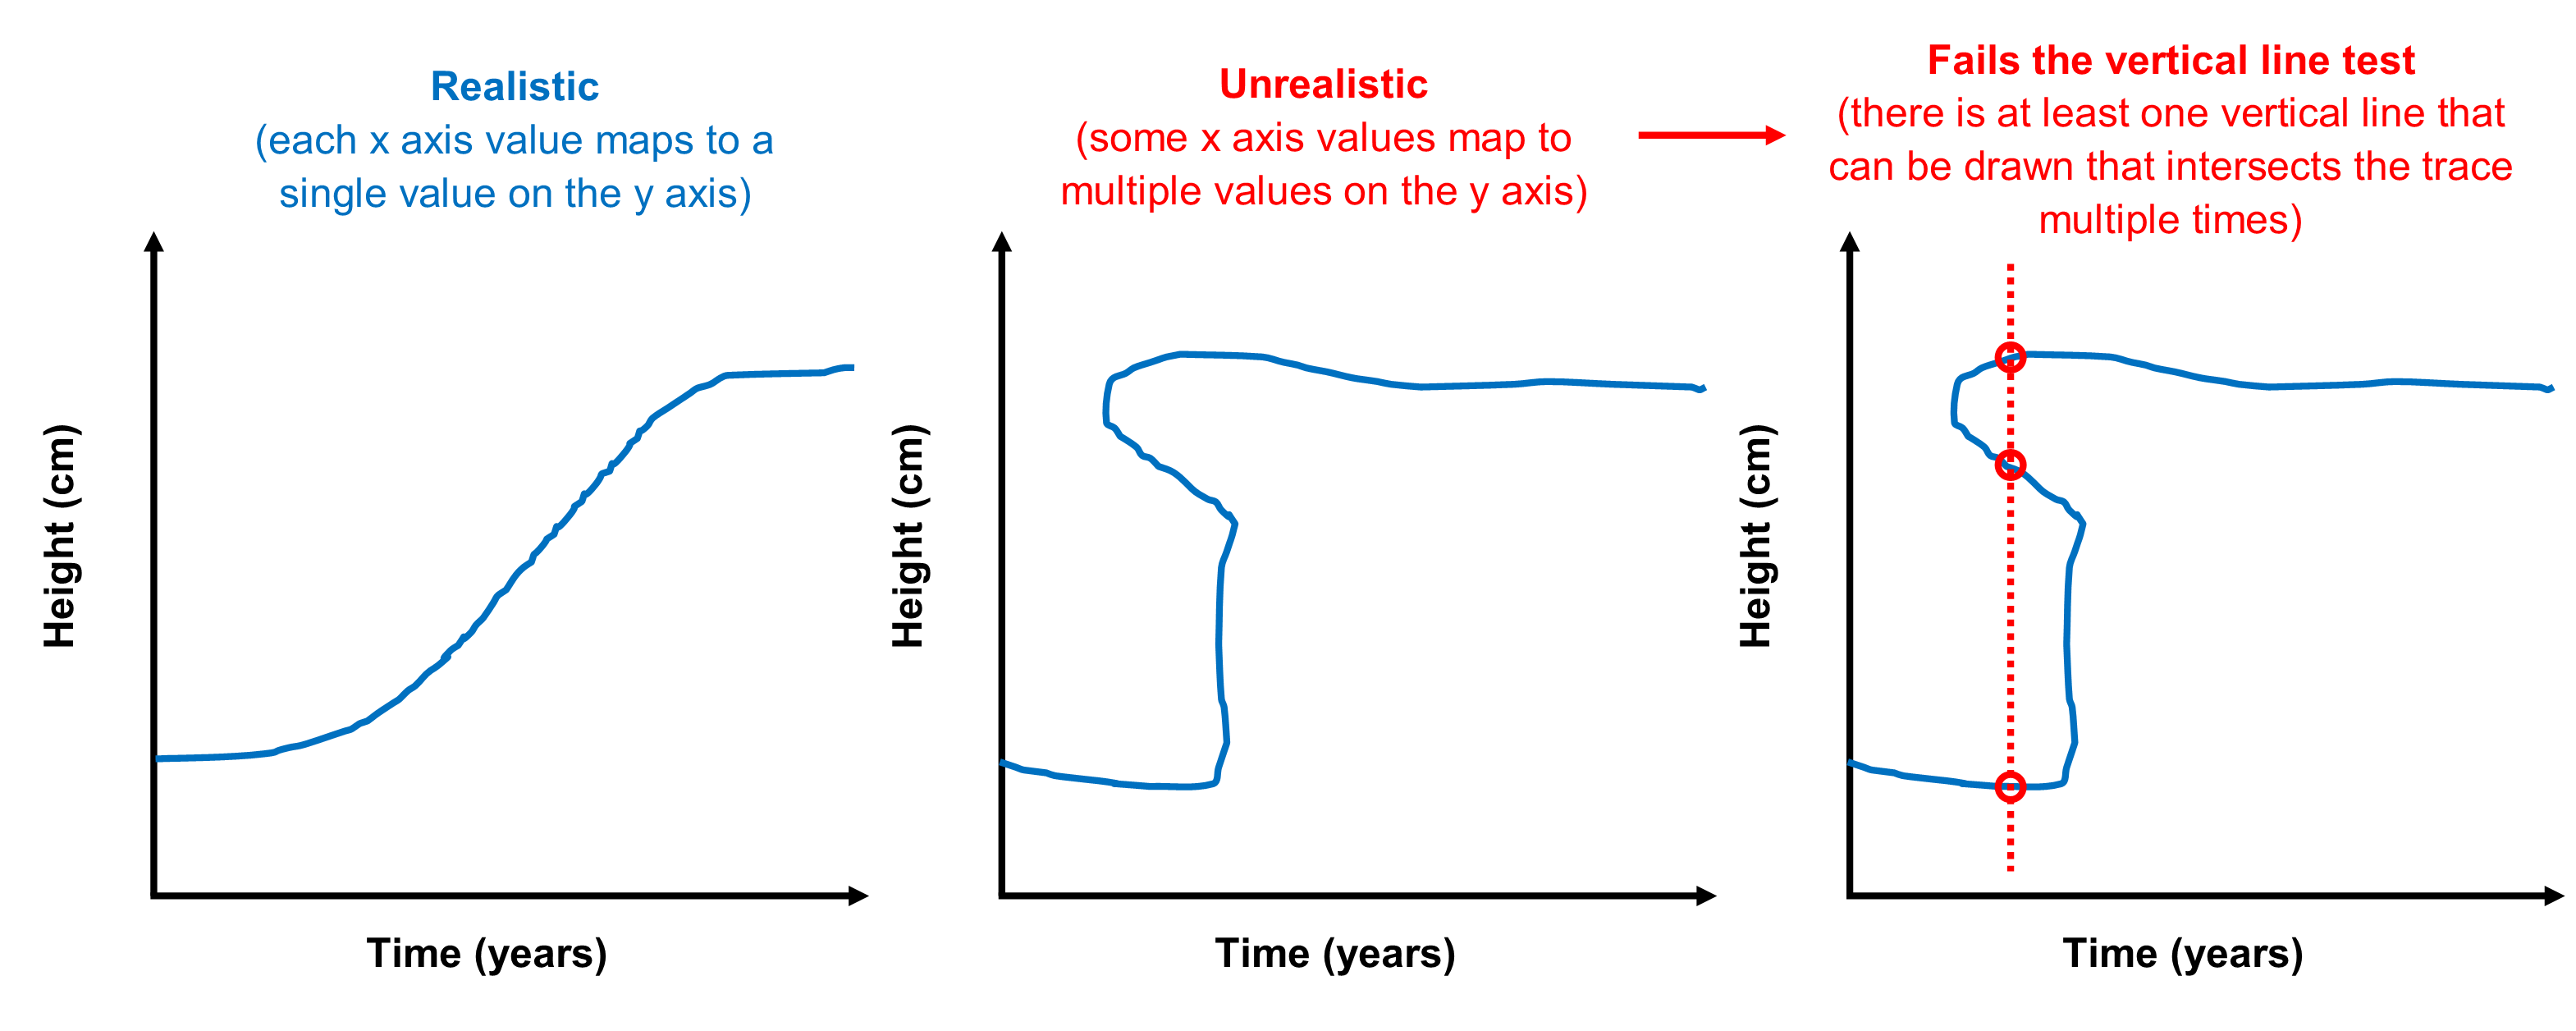
\includegraphics[width=\textwidth]{img/vertical_line/vertical_line_test_mockup.png}
    \caption*{If you plotted your height over time, you would expect each point in time (i.e., each point on the x axis) to correspond to a single height (i.e., a single point on the y axis). The graph on the left matches this expectation and is realistic for this kind of data. The graph in the middle does not match this expectation; there are some points in time that correspond to multiple heights. The graph on the right shows this trace failing the the vertical line test. This is just one of many vertical lines that could be drawn that show that this trace is not a function and thus does not realistically describe data representing height over time.}
\end{figure}

\pagebreak

\subsection*{Data types that should always pass the vertical line test}

Some data types, when plotted, will invariably be functions and thus should always pass the vertical line test. For instance, taking the absorption spectrum of a material should yield one value for absorption for every wavelength. Data types that are always expected to pass the vertical line test include, but are not limited to:

\begin{itemize}
    \setlength\itemsep{-0.5em}
    \item any \href{https://en.wikipedia.org/wiki/Absorption_spectroscopy}{light absorption spectrum}, including ultraviolet-visible (UV-VIS) absorption spectra, infrared (IR) absorption spectra, microwave absorption spectra, X-ray absorption spectra (XAS), etc. (\textit{Note that essentially anything that gets called a ``spectrum" should pass the vertical line test.})
    \item \href{https://en.wikipedia.org/wiki/Nuclear_magnetic_resonance_spectroscopy}{nuclear magnetic resonance (NMR)} spectra
    \item \href{https://en.wikipedia.org/wiki/Electron_paramagnetic_resonance}{electron spin resonance (ESR)/electron paramagnetic resonance (ESR)} spectra
    \item \href{https://en.wikipedia.org/wiki/Fourier-transform_infrared_spectroscopy}{Fourier-transform infrared (FTIR)} spectra
    \item \href{https://en.wikipedia.org/wiki/Raman_spectroscopy}{Raman} spectra
    \item \href{https://en.wikipedia.org/wiki/X-ray_diffraction}{X-ray diffraction (XRD)} patterns/diffractograms
    \item \href{https://en.wikipedia.org/wiki/Energy-dispersive_X-ray_spectroscopy}{energy-dispersive X-ray (EDX/EDS/EDAX)} spectra
    \item \href{https://en.wikipedia.org/wiki/X-ray_photoelectron_spectroscopy}{X-ray photoelectron} spectra (XPS)
    \item \href{https://en.wikipedia.org/wiki/Photoluminescence}{photoluminescence (PL)} spectra
    \item \href{https://en.wikipedia.org/wiki/Mass_spectrometry}{Mass spectra (MS/mass spec)}
    \item \href{https://en.wikipedia.org/wiki/Differential_thermal_analysis}{differential thermal analysis (DTA)} curves
    \item \href{https://en.wikipedia.org/wiki/Differential_scanning_calorimetry}{differential scanning calorimetry (DSC)} curves
    \item \href{https://en.wikipedia.org/wiki/Thermogravimetric_analysis}{thermogravimetric analysis (TGA)} curves
    \item \href{https://en.wikipedia.org/wiki/Transient_photocurrent}{photocurrent response/transient photocurrent (TPC)} curves
    \item \href{https://en.wikipedia.org/wiki/Electroencephalography}{electroencephalograms (EEG)}
    \item \href{https://en.wikipedia.org/wiki/Patch_clamp}{patch-clamp} recordings
\end{itemize}

\subsection*{Data types that may not pass the vertical line test}

For some data types, it is entirely expected that some x axis values will map to multiple y axis values. Data types that may or may not pass the vertical line test include, but are not limited to:

\begin{itemize}
    \setlength\itemsep{-0.5em}
    \item \href{https://en.wikipedia.org/wiki/Cyclic_voltammetry}{cyclic voltammetry (CV)} curves
    \item traces of an object moving in two dimensions, such as a mouse solving a \href{https://en.wikipedia.org/wiki/Morris_water_navigation_task}{Morris water navigation task}
    \item \href{https://en.wikipedia.org/wiki/Pressure%E2%80%93volume_diagram}{Pressure-volume (PV) diagrams}
    \item diagrams of \href{https://en.wikipedia.org/wiki/Graph_theory}{mathematical graphs/networks}
\end{itemize}

\pagebreak

\subsection*{Example 1: Passes the vertical line test}

\href{https://doi.org/10.1021/acsami.4c03997}{Thomas et al. (2024)} report using X-ray diffraction (XRD), Fourier-transform infrared spectroscopy (FTIR) and thermogravimetric analysis (TGA), among other techniques, to characterize kaolinite and kaolinite nanoplatelets. Each of these techniques yield data with one value on the y axis for each value on the x axis. All the plots corresponding to these techniques provided by Thomas et al. pass the vertical line test, as expected.

\begin{figure}[h!tbp]
    \centering
    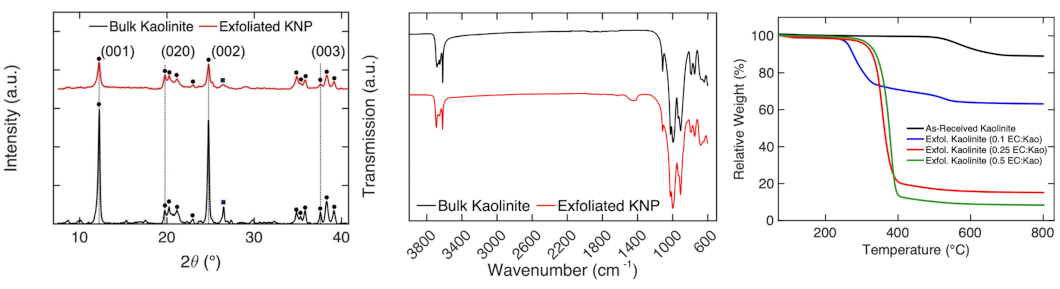
\includegraphics[width=\textwidth]{img/vertical_line/thomas_et_al_mockup.png}
    \caption*{Plots from \href{https://doi.org/10.1021/acsami.4c03997}{Thomas et al. (2024)} that pass the vertical line test (adapted from Figures 2B, S8 and S2).}
\end{figure}

\subsection*{Example 2: Does not pass the vertical line test}

\href{https://doi.org/10.1016/j.ceramint.2014.07.091}{Mandizadeh et al. (2014)} report using FTIR to characterize barium hexaferrite nanostructures. However, the FTIR spectrum they show backtracks on itself several times, failing the vertical line test.

\begin{figure}[h!tbp]
    \centering
    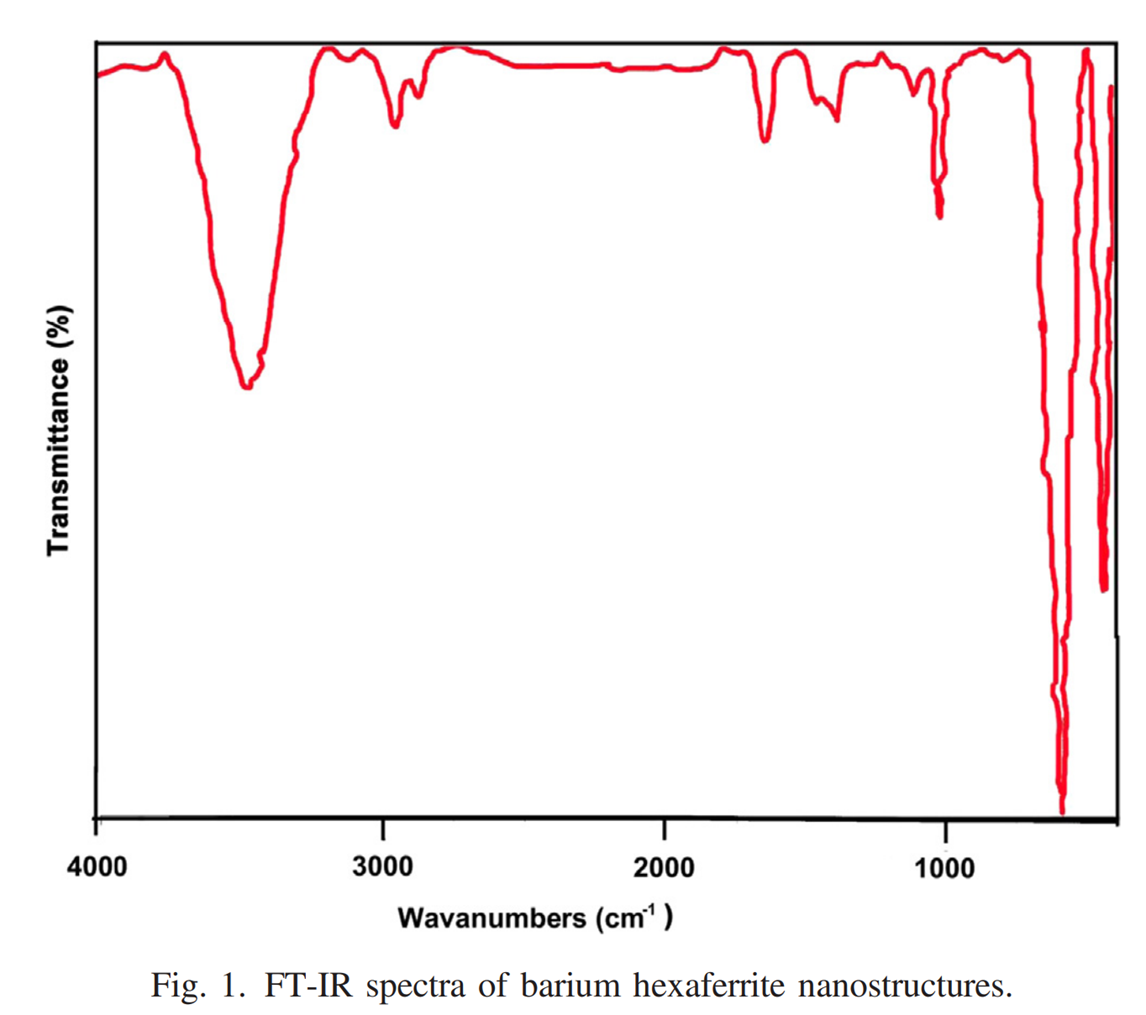
\includegraphics[width=0.6\textwidth]{img/vertical_line/mandizaeh_ftir.png}
    \caption*{An FTIR spectrum from Figure 1 of \href{https://doi.org/10.1016/j.ceramint.2014.07.091}{Mandizadeh et al. (2014)} that fails the vertical line test.}
\end{figure}

\pagebreak

\subsection*{Example 3: Does not pass the vertical line test}

\href{https://doi.org/10.1007/s10854-024-13064-8}{Suguna et al. (2024)} report using FTIR to characterize nanocomposite photocatalysts. However, the FTIR spectra they show appear to be hand-drawn and some fail the vertical line test.

\begin{figure}[h!tbp]
    \centering
    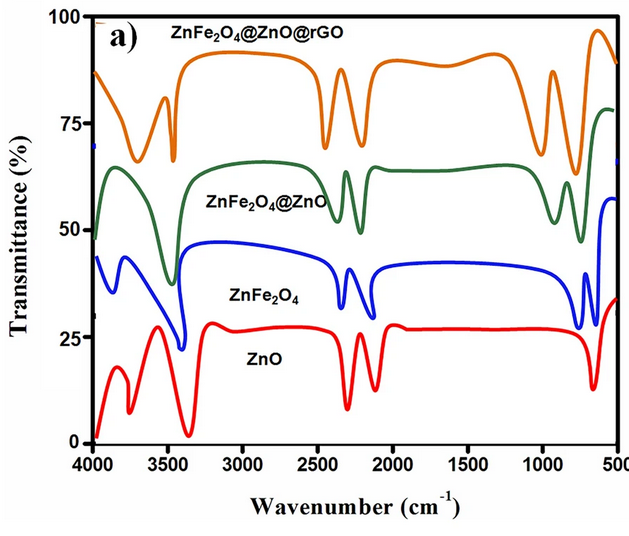
\includegraphics[width=\textwidth]{img/vertical_line/suguna_ftir.png}
    \caption*{FTIR spectra from Figure 3A \href{https://doi.org/10.1007/s10854-024-13064-8}{Suguna et al. (2024)}. The ZnFe$_2$O$_4$ spectrum (in blue) fails the vertical line test.}
\end{figure}

\pagebreak

\subsection*{Example 4: Vertical line test does not apply}

\href{https://doi.org/10.1371/journal.pcbi.1004110}{Lepora and Pezzulo (2015)} describe tracking mice in 2D space. They include several mouse trajectories in figures which follow the path of a mouse with a line. These trajectories are not expected to be functions and thus the vertical line test does not apply.

\begin{figure}[h!tbp]
    \centering
    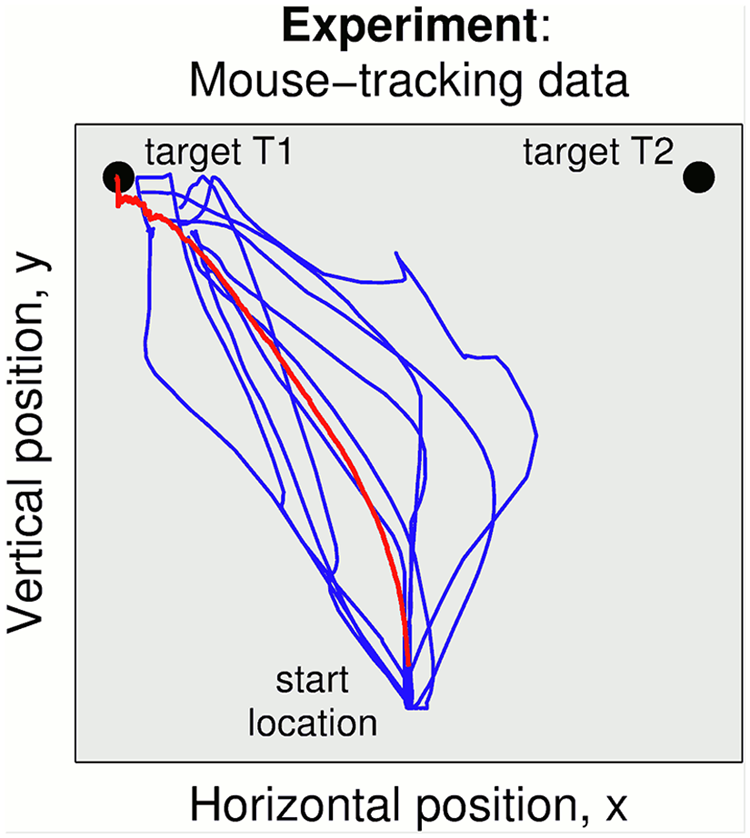
\includegraphics[width=\textwidth]{img/vertical_line/pcbi.1004110.g002.png}
    \caption*{Mouse trajectory traces in 2D space, for which the vertical line test does not apply. Adapted from Figure 2 of \href{https://doi.org/10.1371/journal.pcbi.1004110}{Lepora and Pezzulo (2015)}.}
\end{figure}


\end{document}